	\begin{wrapfigure}[9]{l}{0.14\linewidth}
		%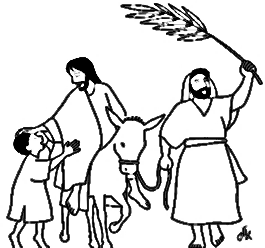
\includegraphics{foule_rameaux.png}
		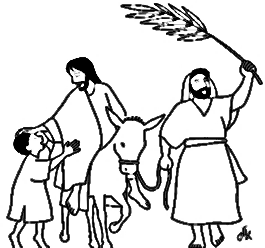
\includegraphics[width=1.4\linewidth]{foule_rameaux.png}
	\end{wrapfigure}
La procession de ce jour n’est pas un cortège funèbre - c’est
une marche victorieuse : GLOIRE, HONNEUR, LOUANGE... La
palme, symbole du triomphe, et l’olivier, signe de paix, sont
agités avec des \og Hosanna ! \fg de joie.
La liturgie n’entend pas rejouer un drame historique. Elle
célèbre le Christ présent au milieu de nous, et ce Christ ne
souffre plus, ne meurt plus. Il est vivant, ressuscité.
Dans cette procession l’Eglise acclame le Christ d’aujourd’hui.
Ce dimanche ouvre la Semaine Sainte. La fête des Rameaux commémore deux
évènements contrastés : l’entrée triomphale de Jésus à Jérusalem et sa passion et
sa mort sur la Croix. Les deux évènements sont intimement liés l’un à l’autre.
Jésus est accueilli triomphalement par une foule enthousiaste qui le reconnaît
comme le Messie, le nouveau roi d’Israël, celui qui vient apporter la libération au
nom du Seigneur. C’est ce qui explique l’usage des rameaux, ces palmes de
victoire et les cris de joie du peuple accompagnés de la fameuse acclamation
"Hosanna" au fils de David qu’il faut traduire par \og aide-nous \fg
Quelques jours plus tard, la foule changera comme une girouette et criera :
Crucifie-le ! Les chefs religieux, eux, auront la terrible logique de leur haine, une
haine sacrée - pour protéger leur intérêt ! C’est ici que nous comprenons la
froideur et la mesquinerie, l’hypocrisie et la méchanceté des hommes. Si Jésus a
été condamné, c’est parce que les hommes ont préféré les sacrifices de la loi à la
miséricorde, de la vérité au mensonge, les ténèbres à la lumière. Pourtant, celui
qui couvre la vérité enfante le mensonge, nous dit le psalmiste.

\begin{wrapfigure}{l}{1.3cm}
\vspace{-0.5cm}
	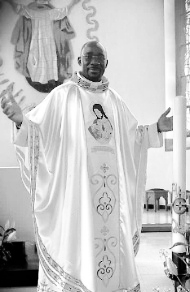
\includegraphics{standing_daniel.png}
\end{wrapfigure}

Autrement dit,
celui qui ne choisit pas l’amour finit par devenir complice du
mal. Tout au long de cette Semaine Sainte, accrochons-nous
à la Parole de Dieu et suivons le Christ dans ces diverses
étapes : Jeudi Saint, nous célèbrerons l’Institution de
l’Eucharistie et du Sacerdoce ; Vendredi Saint, nous
suivrons Jésus jusqu’aux pieds de la Croix. Samedi Saint,
à la Veillée Pascale, nous célèbrerons sa victoire sur la mort.
\begin{flushright}
Bonne méditation !
\textit{Père  Daniel  ETTÉ}
\end{flushright}

